\documentclass[xcolor=dvipsnames,10pt]{beamer}
\usepackage[english]{babel}
\usepackage[utf8]{inputenc}
\usepackage{pict2e}
\usepackage{colortbl}
\usepackage{graphicx}
\usepackage{pdfpages}
\usepackage{verbatim}
\usepackage{pgf}
%%%%%%%%%%%%%%%%%%%%
%%% nice math
\usepackage{amssymb}
\usepackage{amsmath}
\usepackage{latexsym}
\usepackage{amsthm}
\usepackage{slashed}
%%%%%%%%%%%%%%%%%%%%
%%% font type
%\usepackage{times}
\usepackage{bookman}
%\usepackage{palatino}
%\usepackage{newcent}
%\usepackage{avant}
\usefonttheme{serif}
\usepackage{atlasphysics}
%\usepackage{tikz}
\usepackage{subfigure}

\newcommand{\AC}{\ensuremath{\text{A}_{\text{C}}}}
\newcommand{\formatGenerator}[1]{\textsc{#1}}
\newcommand{\mcnlo}{\formatGenerator{mc@nlo}}
\newcommand{\wjets}{\ensuremath{W+\mathrm{jets}}}
\providecommand{\abs}[1]{\lvert#1\rvert}
\newcommand{\dy}{\ensuremath{\Delta{}\abs{y}}}
\newcommand{\deta}{\ensuremath{\Delta{}\abs{\eta}}}
\newcommand{\mtt}{\ensuremath{m_{\ttbar{}}}}
\newcommand{\Nupup}{\ensuremath{N(\uparrow\uparrow)}}
\newcommand{\Ndodo}{\ensuremath{N(\downarrow\downarrow)}}
\newcommand{\Nupdo}{\ensuremath{N(\uparrow\downarrow)}}
\newcommand{\Ndoup}{\ensuremath{N(\downarrow\uparrow)}}


\newcommand\myskip{\vspace{\baselineskip}}
\def\Xbar{\ensuremath{\bar{X}}}
\def\XXbar{\antibar{X}}
\def\Ybar{\ensuremath{\bar{Y}}}
\def\YYbar{\antibar{Y}}
\def\Tbar{\ensuremath{\bar{T}}}
\def\TTbar{\antibar{T}}
\def\Bbar{\ensuremath{\bar{B}}}
\def\BBbar{\antibar{B}}
\newcommand\TT{\ensuremath{T\bar{T}}}
\newcommand\BB{\ensuremath{B\bar{B}}}
\newcommand\T{\ensuremath{T}}
\newcommand\B{\ensuremath{B}}
\newcommand{\TB}{\ensuremath{(T \, B)}}
\newcommand{\XT}{\ensuremath{(X \, T)}}
\newcommand{\BY}{\ensuremath{(B \, Y)}}
\def\Tlr{\ensuremath{T_{L,R}}}
\def\Blr{\ensuremath{B_{L,R}}}
\def\Ylr{\ensuremath{Y_{L,R}}}
\def\Xlr{\ensuremath{X_{L,R}}}
\def\TBlr{\ensuremath{\TB_{L,R}}}
\def\BYlr{\ensuremath{\BY_{L,R}}}
\def\XTlr{\ensuremath{\XT_{L,R}}}
\def\vlt{vector-like top partner}
\def\vlb{vector-like bottom partner}

%%%%%%%%%%%%%%%%%%%%%%%%
%%% LAZYNESS-DRIVEN DEFS
%%%%%%%%%%%%%%%%%%%%%%%%
\def\cme{center-of-mass energy}
\def\cmm2{cm$^{-2}$}
\def\sm1{s$^{-1}$}
\def\chisq{$\chi^2$}
\def\loose{{\sc Loose}}
\def\tight{{\sc Tight}}
\def\whad{\ensuremath{W_{\rm had}}}
\def\wlep{\ensuremath{W_{\rm lep}}}
\def\wi{$W_{\rm had}^{\rm type\;I}$}
\def\wii{$W_{\rm had}^{\rm type\;II}$}
\def\mreco{\ensuremath{m_{\rm reco}}}
\def\chii{{\sc ``{\small 2 \btag ged jets}''}}
\def\chiii{{\sc ``{\small 3 \btag ged jets}''}}
\def\chiv{{\sc ``{\small{\footnotesize$\geq$}4 \btag ged jets}''}}

\def\dr{\ensuremath{\Delta R}}
\def\OR{\texttt{OR}}
\def\AND{\texttt{AND}}
%\def\bjet{$b$jet}
\def\bjet{$b$-jet}
%\def\cjet{$c$jet}
\def\cjet{$c$-jet}
\def\ljet{light-jet}
\def\btag{$b$-tag}
\def\ctag{$c$-tag}
\def\mt{\ensuremath{m_T}}
\def\mtw{\ensuremath{m_T(W)}}
\def\wbx{\ensuremath{\TTbar\to Wb+X}}
\def\htx{\ensuremath{\TTbar\to Ht+X}}
\def\nontt{non-$t\bar{t}$}
\def\mclimit{\texttt{MCLimit}}
\def\cls#1{\ensuremath{CL_{\rm #1}}}
\def\hthad{\ensuremath{H_T^{\rm had}}}
\def\htfj{\ensuremath{H_T^{4j}}}
\def\tthf{\ttbar+HF}
\def\ttlf{\ttbar+light}

\def\bra#1{\mathinner{\langle{#1}|}}
\def\ket#1{\mathinner{|{#1}\rangle}}
\def\braket#1{\mathinner{\langle{#1}\rangle}}
\def\Bra#1{\left<#1\right|}
\def\Ket#1{\left|#1\right>} 
\newcommand{\Overline}[2][1]{%
  {}\mkern#1mu \overline{\mkern-#1mu #2 \mkern-#1mu}\mkern#1mu {}} 
\DeclareMathAlphabet{\mathpzc}{OT1}{pzc}{m}{it}



%%% nice tables
\usepackage{booktabs}
\usepackage{multirow}

\usepackage{fancybox}

%%% code pieces
\usepackage{listings}
\lstset{basicstyle=\tiny,language=c,emphstyle=\color{red},columns=fullflexible,
keepspaces=false, keywordstyle=\tiny\color{blue}, showstringspace=false} 
\newcommand\BackgroundPicture[1]{%
   \setbeamertemplate{background}{%
   \parbox[c][\paperheight]{\paperwidth}{%
       \vfill \hfill
\includegraphics[width=0.6\paperwidth,height=0.6\paperheight]{#1}
        \hfill \vfill
     }}}

%\setbeamertemplate{headline}

%%% to allow small margin
\newenvironment{changemargin}[2]{%
  \begin{list}{}{%
    \setlength{\topsep}{0pt}%
    \setlength{\leftmargin}{#1}%
    \setlength{\rightmargin}{#2}%
    \setlength{\listparindent}{\parindent}%
    \setlength{\itemindent}{\parindent}%
    \setlength{\parsep}{\parskip}%
  }%
  \item[]}{\end{list}} 

%\usetheme{Luebeck}
%\usecolortheme{seagull}
%\usecolortheme[named=BrickRed]{structure}


\usetheme[headheight=.13\textheight,footheight=.035\textheight]{boxes}
\definecolor{light-gray}{gray}{0.9}
%\definecolor{myfading}{fg=white,bg=light-gray}
\definecolor{structure2}{rgb}{1,1,1}

\mode<presentation>
%\usecolortheme[named=Black]{structure}
%\usecolortheme[named=Plum]{structure}
%\usecolortheme[named=Violet]{structure}
%\usecolortheme[named=BurntOrange]{structure}
%\usecolortheme[named=RedViolet]{structure}
\usecolortheme[named=Sepia]{structure}
\setbeamercolor{normal text}{fg=black!70!light-gray,bg=white}
\setbeamercolor{alerted text}{fg=BrickRed,bg=light-gray}
\setbeamercolor{boxcolor}{fg=black!70!light-gray,bg=structure!30!white}
\setbeamercolor{whiteboxcolor}{fg=black!70!light-gray,bg=white}

\definecolor{links}{named}{Plum}

\usepackage{hyperref}
\hypersetup{colorlinks=true,linkcolor=,urlcolor=links}

\setbeamercolor{head/foot boxes}{fg=structure!90!white,bg=structure!30!white}
\setbeamercolor{head/foot boxes bis}{fg=structure!60!white,bg=structure!90!white}

\setbeamercolor{head/foot text}{fg=structure!40!black,bg=structure!30!white}

%\addheadboxtemplate{\usebeamercolor[bg]{head/foot boxes}}{\usebeamercolor[fg]{head/foot text}\logo{
\includegraphics[height=1.2cm]{pics/atlasifae2}}\raisebox{-1.8ex}{\insertlogo}\hfill\insertshorttitle \hskip0.3cm}
\addheadboxtemplate{\usebeamercolor[bg]{head/foot boxes}}{\usebeamercolor[fg]{head/foot text}\insertsubsectionhead \hskip0.3cm}
\addheadboxtemplate{\usebeamercolor[fg]{head/foot boxes}}{\usebeamercolor[bg]{head/foot text}\scriptsize\hskip0.3cm\insertsectionhead}

\addfootboxtemplate{\usebeamercolor[fg]{head/foot boxes}}{\usebeamercolor[bg]{head/foot text}\hskip0.3cm\insertshortauthor\\\insertshortinstitute \hfill}
\addfootboxtemplate{\usebeamercolor[fg]{head/foot boxes bis}}{\usebeamercolor[fg]{head/foot text}\hfill\insertdate\hfill}

\def\insertpresentationendframe{\inserttotalframenumber}
\makeatletter
\g@addto@macro{\appendix}{\immediate\write\@auxout{\string\@writefile{nav}{\noexpand\headcommand{\noexpand\def\noexpand\insertpresentationendframe{\the\c@framenumber}}}}}
\makeatother

\addfootboxtemplate{\usebeamercolor[bg]{head/foot boxes}}{\usebeamercolor[fg]{head/foot text}\hfill\insertframenumber/\insertpresentationendframe\hskip0.3cm}
%\addfootboxtemplate{\usebeamercolor[bg]{head/foot boxes}}{\usebeamercolor[fg]{head/foot text}\hfill\insertframenumber/\insertpresentationendpage\hskip0.3cm}

%\setbeamertemplate{footline}{%
%  \begin{beamercolorbox}{section in head/foot}
%\begin{center}
%\begin{tabular}{lcr}
%\hskip45pt \textit{Barcelona plans for u4u4 searches in lepton+jets} \phantom{a/aa} & 2011, December 21st \phantom{a/aa} \insertframenumber / %\insertpresentationendpage
%\\
%\end{tabular}
%\end{center}  \end{beamercolorbox}
%}


%\usesectionheadtemplate
%{\color{white}\tiny\textbf{\insertsectionhead}}
%{\color{structureshaded}\tiny\textbf{\insertsectionhead}}


%\useoutertheme{sidebar}
%\setbeamertemplate{sidebar canvas left}[vertical shading][top=White,bottom=Gray]
%\setbeamertemplate{sidebar canvas left}[vertical shading][top=White,bottom=CadetBlue]
%\setbeamertemplate{sidebar canvas left}[vertical shading][top=White,bottom=YellowGreen]
%\setbeamertemplate{sidebar canvas left}[vertical shading][top=White,bottom=light-gray]

\setbeamertemplate{navigation symbols}{}
\setbeamersize{text margin left=.2cm,text margin right=.2cm} 






\AtBeginSection[]
{
  \begin{frame}\centering
    \frametitle{Outline}
    \tableofcontents[currentsection]
  \end{frame}
}



\title[Probing new physics at the LHC: \\ searches for heavy top-like quarks \\ with the ATLAS experiment]{{\bfseries Probing new physics at the LHC: \\ searches for heavy top-like quarks \\ with the ATLAS experiment}}
\author[A Succurro]{Antonella Succurro\\ \vspace{\baselineskip}\textit{\small PhD candidate in Physics}\vspace{-0.7cm}}
\institute[\, \emph{IFAE, UAB}]{
\begin{tabular}{p{0.25\textwidth} p{0.25\textwidth} p{0.25\textwidth}}
  \vspace{0.7cm} 
\includegraphics[width=2.5cm]{../smallstuff/ifae_logo.pdf}\hspace{0.2cm}&
  \vspace{0.5cm} 
\includegraphics[width=2.8cm]{../smallstuff/uab_logo.pdf}&
  \vspace{0.cm} \hspace{0.5cm} 
\includegraphics[width=1.5cm]{pics/atlas_logo}\\
\end{tabular}
}
\date{Bellaterra, 28th of February, 2014}


\begin{document}

\frame{

\vspace{-.8cm}


\maketitle\centering

\vspace{-.8cm}



}

%\begin{frame}\frametitle{Content}
%\end{frame}
%\begin{frame}\frametitle{Outline}
%\centering
%\tableofcontents[part=1,pausesections]
%\tableofcontents
%\end{frame}

%----------------------------------
\section{Introduction}
%----------------------------------

\begin{frame}\frametitle{Standard Model as an effective theory}
\scriptsize\centering

\myskip
\end{frame}




%----------------------------------
\section{Theoretical framework}
%----------------------------------


%----------------------------------
\section{The ATLAS experiment at the LHC}
%----------------------------------

\BackgroundPicture{../detector/figures/atlas}

\begin{frame}\frametitle{The ATLAS Detector}
\footnotesize\centering

\footnotesize
\begin{minipage}{.35\textwidth}
A general purpose experiment
\begin{itemize}
\item vertex detector and central tracker
\item superconducting solenoid
\item electromagnetic and hadronic calorimeters
\item muon spectrometer
\item superconducting toroids
\item high hermeticity (full $\phi$ and $|\eta|<5$)
%\item fake electrons and photons rejection (rejection rate of 10$^5$ and 10$^3$)
%\item very selective and efficient trigger (rejection rate of 10$^7$)
\end{itemize}
%\vspace{1.5cm}
\end{minipage}\begin{minipage}{.6\textwidth}\centering\pause
\hspace{2cm}\begin{beamercolorbox}[wd=.9\textwidth,rounded=true,shadow=true]{whiteboxcolor}\centering
{\bfseries In 2012 21.7\ifb\  collected at $\sqrt{s}=8~$TeV!}
\vspace{.3cm}

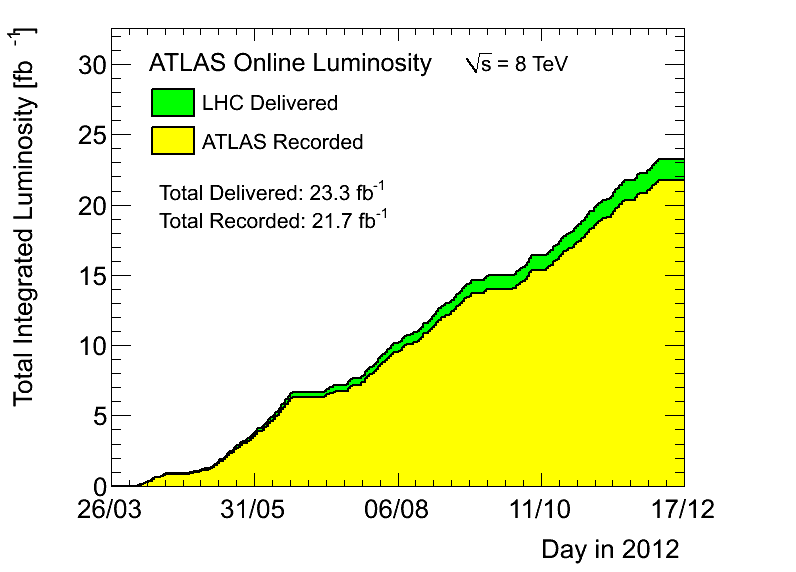
\includegraphics[width=.8\textwidth]{pics/sumLumiByDay2012}

\vspace{\baselineskip}
%Reached peak luminosity of $3.65\times 10^{33}~$cm$^{-2}$s$^{-1}$\\
\end{beamercolorbox}

See \href{https://twiki.cern.ch/twiki/bin/view/AtlasPublic}{ATLAS public page}

\end{minipage}

\myskip
Will present results obtained with \alert{14.3\ifb}\ of 2012 data

\end{frame}

\BackgroundPicture{pics/emptyIMG}




%----------------------------------
\section{Monte Carlo simulation}
%----------------------------------

\begin{frame}\frametitle{Modelling of hadron collisions}
\small\centering

want to do physics at hadron colliders?

need a good understanding of incoming hadrons

\myskip
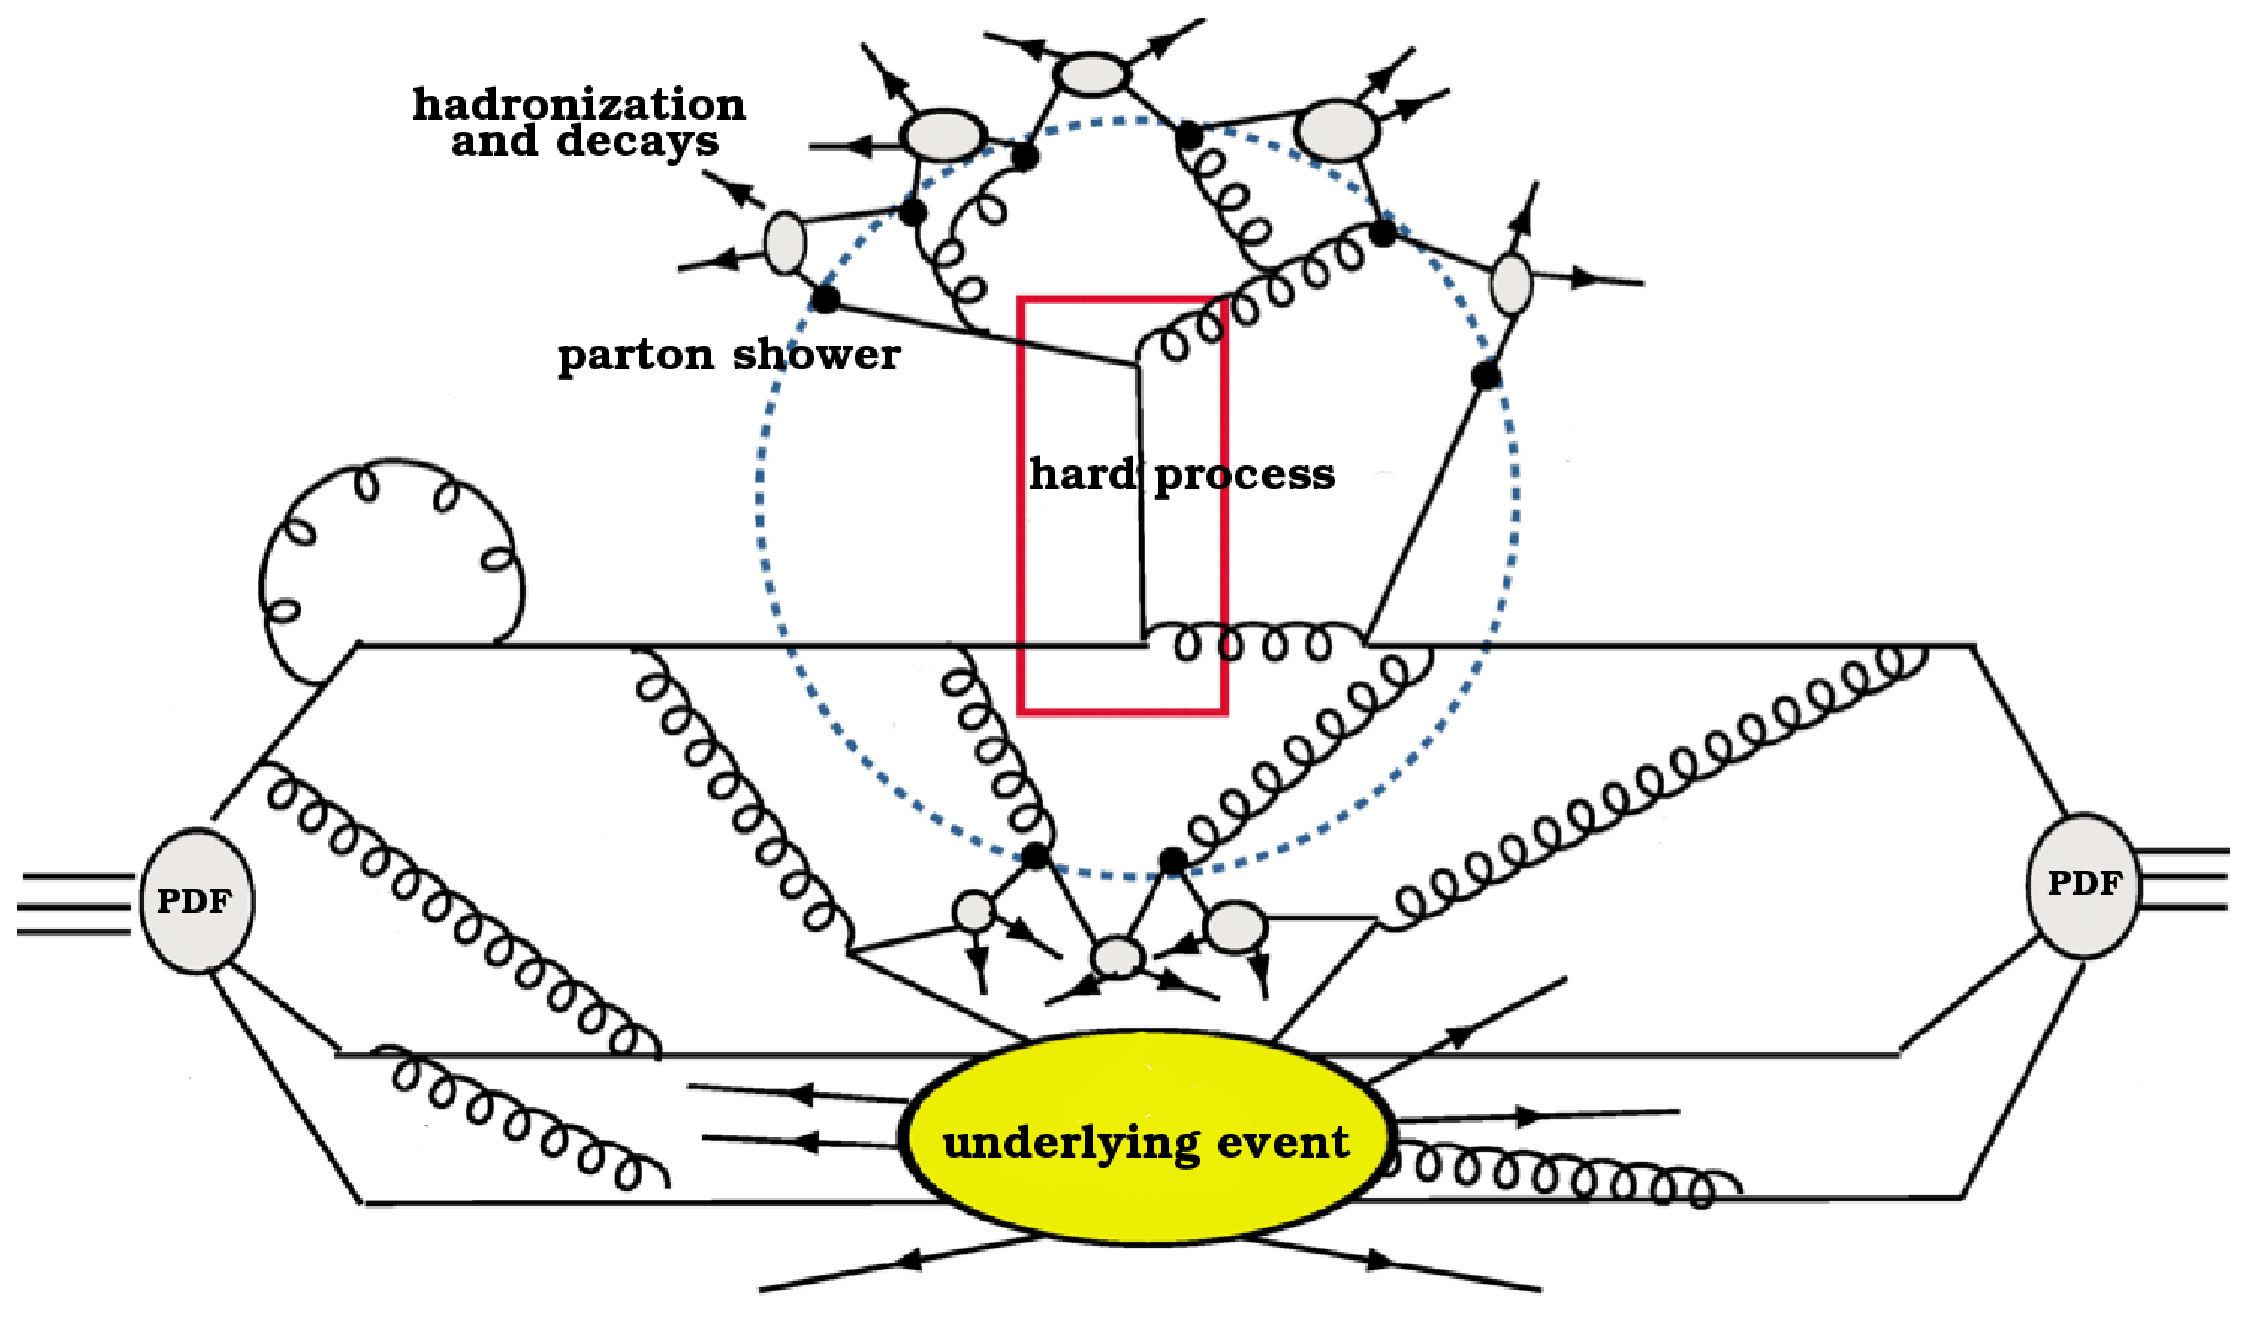
\includegraphics[width=.7\textwidth]{../montecarlo/figures/my_collision}

\end{frame}


\begin{frame}\frametitle{Modelling of hadron collisions}
\centering\myskip
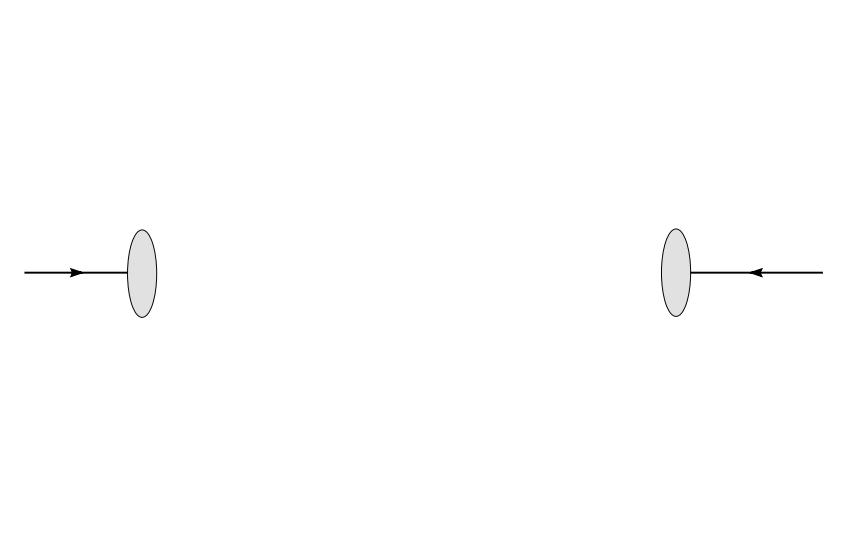
\includegraphics[height=0.8\textheight]{../montecarlo/figures/event1}

\begin{flushright}\tiny Drawings from~\cite{Gieseke}\end{flushright}

\end{frame}


\begin{frame}\frametitle{Hard scattering of two partons}
\centering\myskip
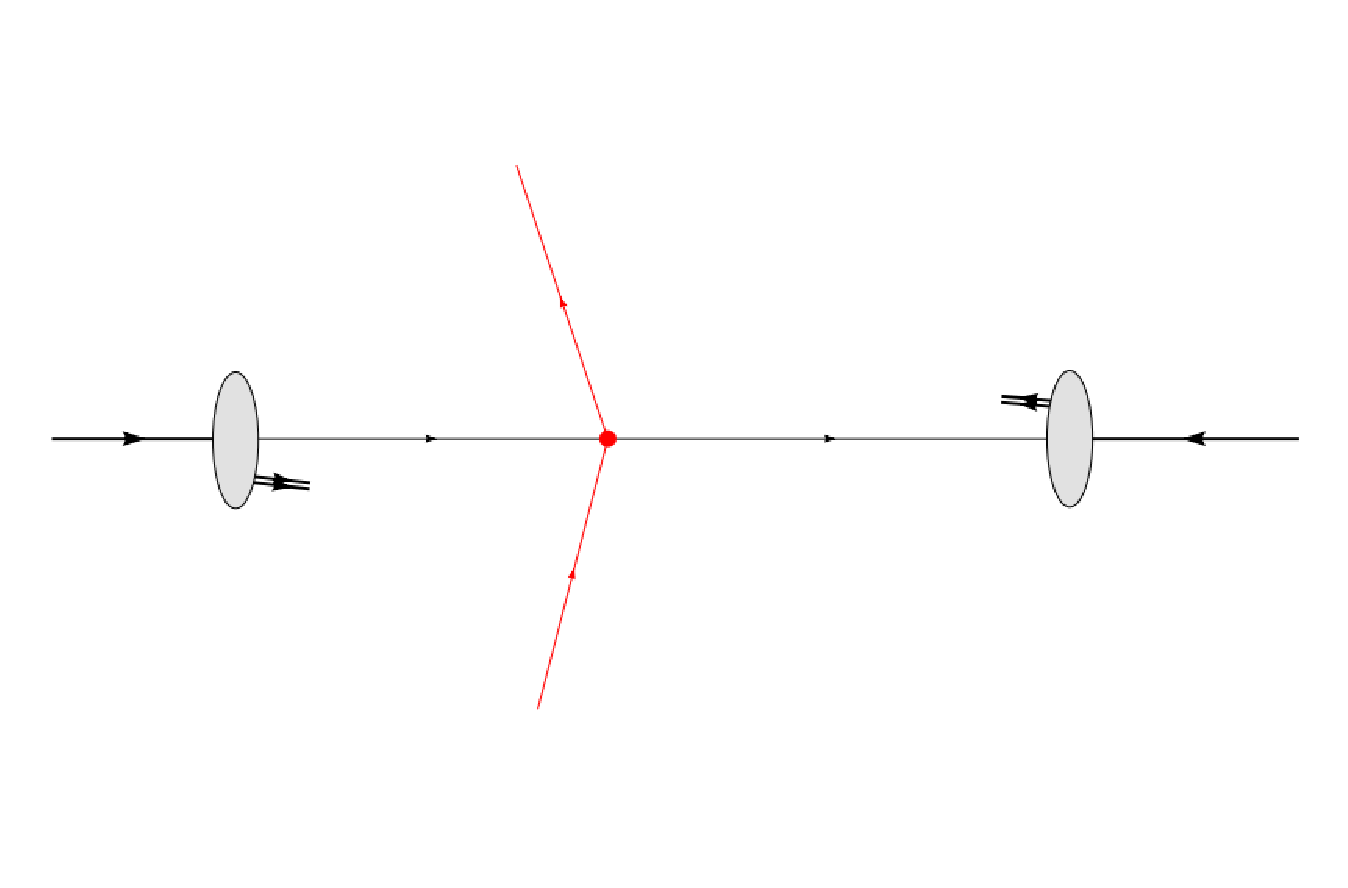
\includegraphics[height=0.8\textheight]{../montecarlo/figures/event2}

\begin{flushright}\tiny Drawings from~\cite{Gieseke}\end{flushright}

\end{frame}

\begin{frame}\frametitle{Parton showering}
\centering\myskip
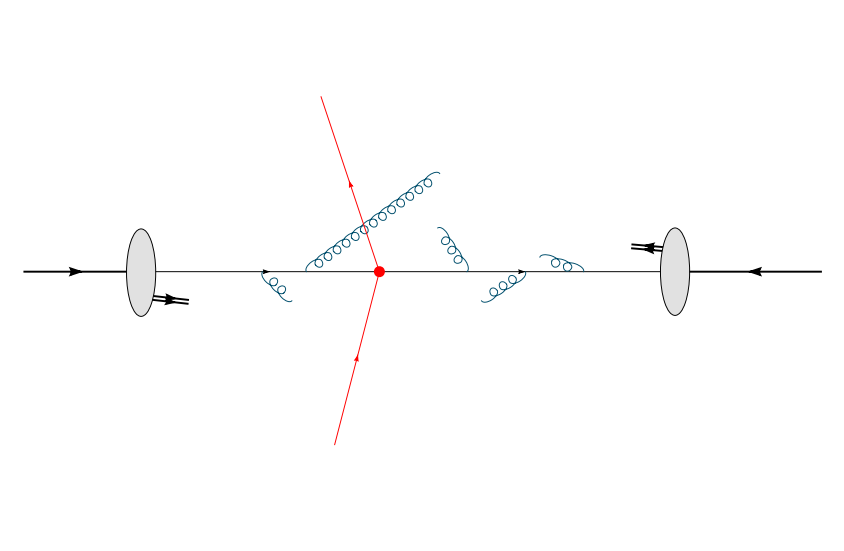
\includegraphics[height=0.8\textheight]{../montecarlo/figures/event3}

\begin{flushright}\tiny Drawings from~\cite{Gieseke}\end{flushright}

\end{frame}

\begin{frame}\frametitle{Parton showering}
\centering\myskip
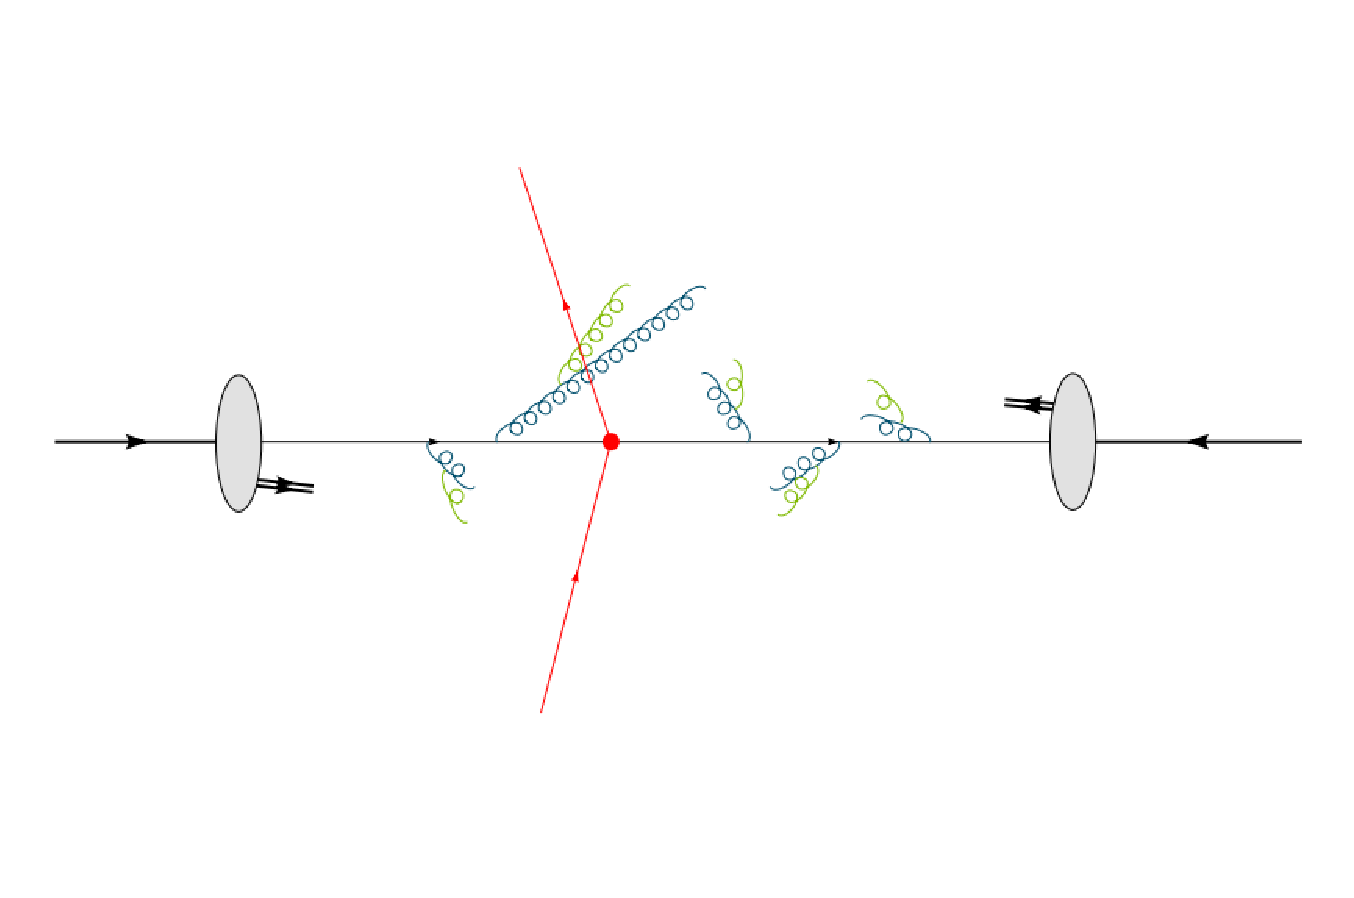
\includegraphics[height=0.8\textheight]{../montecarlo/figures/event4}

\begin{flushright}\tiny Drawings from~\cite{Gieseke}\end{flushright}

\end{frame}

\begin{frame}\frametitle{Hadronization}
\centering\myskip
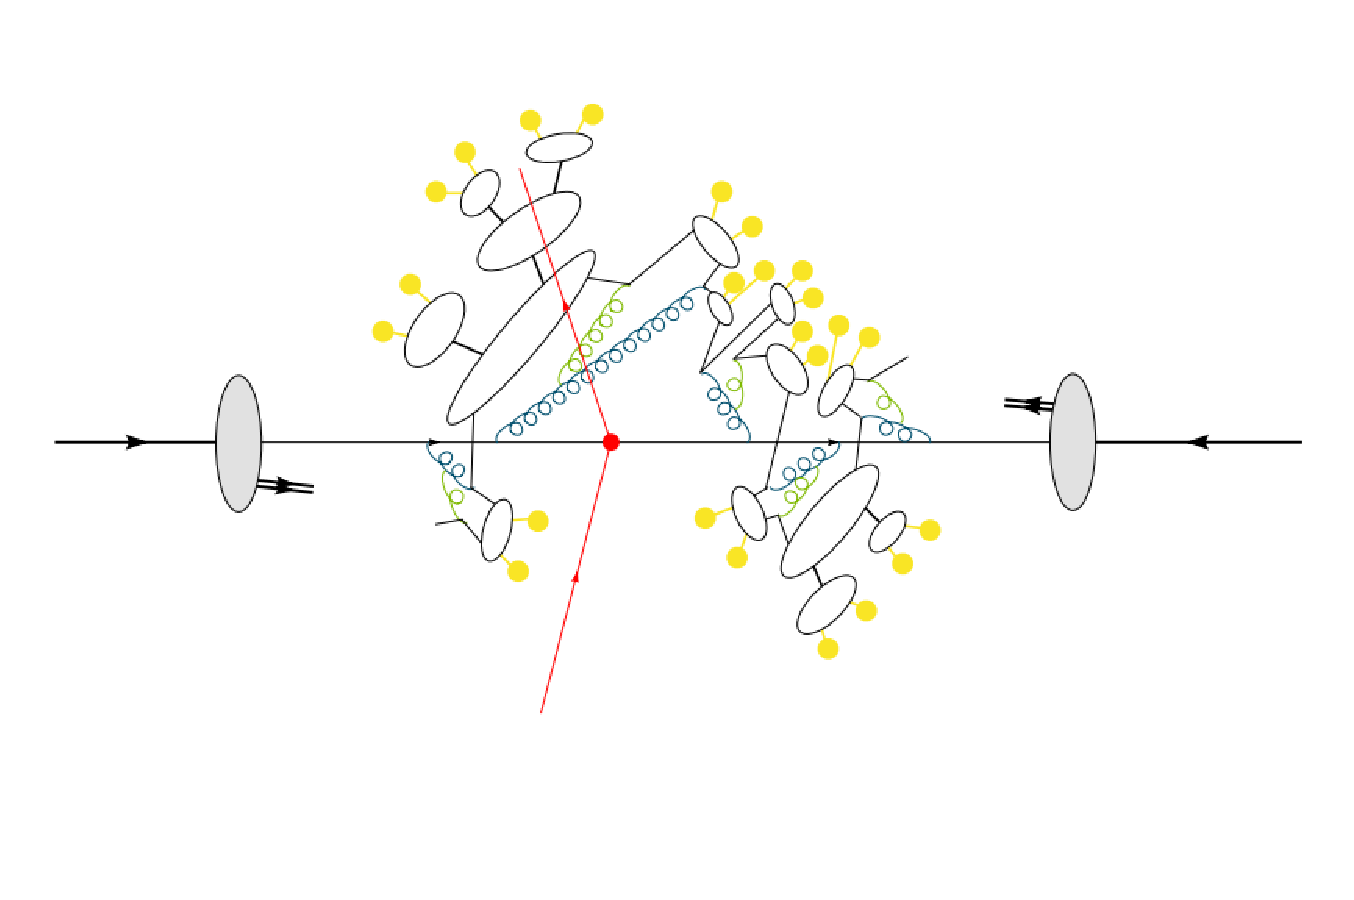
\includegraphics[height=0.8\textheight]{../montecarlo/figures/event5}

\begin{flushright}\tiny Drawings from~\cite{Gieseke}\end{flushright}

\end{frame}

\begin{frame}\frametitle{Final particle decays}
\centering\myskip
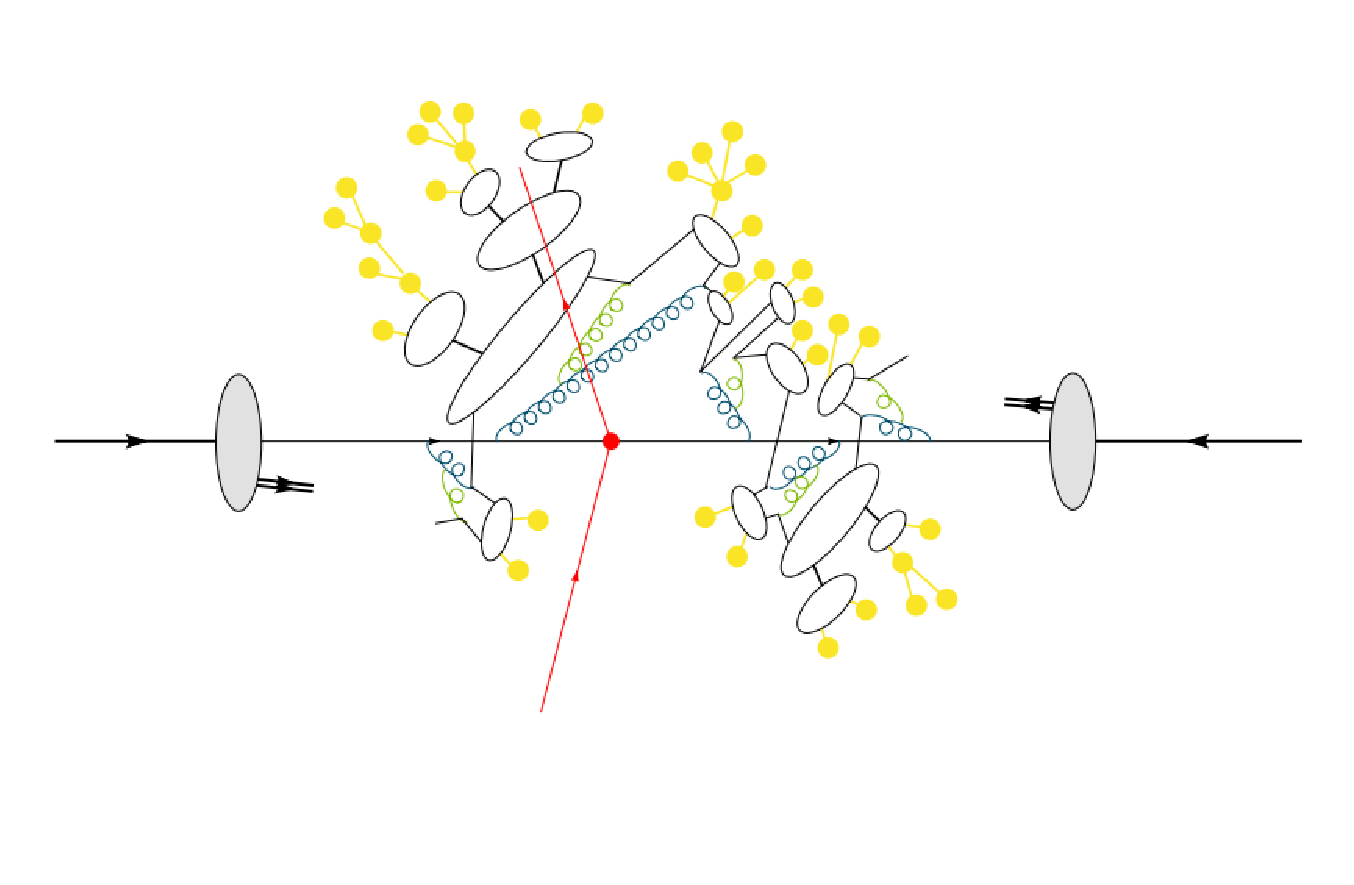
\includegraphics[height=0.8\textheight]{../montecarlo/figures/event6}

\begin{flushright}\tiny Drawings from~\cite{Gieseke}\end{flushright}

\end{frame}

\begin{frame}\frametitle{Underlying event simulation}
\centering\myskip
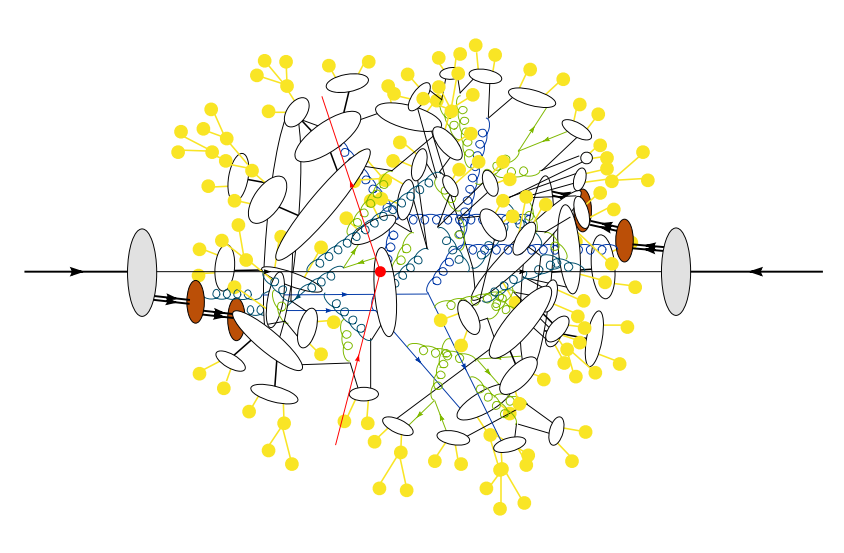
\includegraphics[height=0.8\textheight]{../montecarlo/figures/event7}

\begin{flushright}\tiny Drawings from~\cite{Gieseke}\end{flushright}

\end{frame}


%----------------------------------
\section{Event reconstruction}
%----------------------------------

%----------------------------------
\section{Searches for vector-like top partner pairs in the single lepton channel}
%----------------------------------

%----------------------------------
\section{Search for \TTbar\ decaying to $Wb+X$}
%----------------------------------

%----------------------------------
\section{Search for \TTbar\ decaying to $Ht+X$}
%----------------------------------

%----------------------------------
\section{Final results}
%----------------------------------

%----------------------------------
\section{Conclusions and outlook}
%----------------------------------


\appendix


\section*{References}
\setbeamertemplate{bibliography item}[text]

\begin{frame}[allowframebreaks]
\frametitle{References}\footnotesize
\bibliographystyle{unsrt}
%\bibliographystyle{myunsrt}
\bibliography{heavyquarks.bib}
\end{frame}


\section*{Backup}

%----------------------------------
\begin{frame}
 \frametitle{}

\begin{center}{\bfseries
BACKUP SLIDES}
\end{center}
\end{frame}





\end{document}
